\documentclass[a4paper, 12pt]{article}

% =================================================================================
% 1. UNIVERSAL PREAMBLE & PACKAGES
% =================================================================================
\usepackage[margin=2cm]{geometry}
\usepackage{fontspec}
\usepackage{amsmath}
\usepackage{amssymb}
\usepackage{graphicx}
\usepackage{enumitem}
\usepackage{parskip}
\usepackage{multicol}

% Language Setup
\usepackage[indonesian, provide=*]{babel}
\babelprovide[import, onchar=ids fonts]{indonesian}
\babelprovide[import, onchar=ids fonts]{english}

% Fonts
\babelfont{rm}{Noto Sans}
\babelfont{sf}{Noto Sans}

% Graphics & TikZ
\usepackage[most]{tcolorbox}
\usepackage{tikz}
\usetikzlibrary{
    shapes, shapes.symbols, shapes.geometric, 
    arrows.meta, positioning, calc, 
    shadows, backgrounds, patterns, 
    decorations.pathreplacing
}

% =================================================================================
% 2. COLOR DEFINITIONS (MERGED FROM ALL SOURCES)
% =================================================================================

% --- Palette 1: Teori Dasar ---
\definecolor{mainBlue}{HTML}{2C3E50}
\definecolor{accentTeal}{HTML}{16A085}
\definecolor{alertRed}{HTML}{E74C3C}
\definecolor{niceOrange}{HTML}{F39C12}
\definecolor{powerBlue}{HTML}{2980B9}
\definecolor{cubeRed}{HTML}{C0392B}
\definecolor{softBgA}{HTML}{ECF0F1}
\definecolor{softBgB}{HTML}{F7F9F9}
\definecolor{solGreen}{HTML}{27AE60}
\definecolor{lightPurple}{HTML}{9B59B6}

% --- Palette 2: Soal 1-5 (Pastel) ---
\definecolor{colP}{RGB}{100, 149, 237}     % Biru
\definecolor{colQ}{RGB}{255, 179, 71}      % Oranye
\definecolor{colR}{RGB}{60, 179, 113}      % Hijau
% colGray defined below in Palette 3 usually works for both, but defined here if needed separate:
\definecolor{colGrayMid}{RGB}{220, 220, 220} 

% --- Palette 3: Soal 6-10 (Ramah Anak) ---
\definecolor{colBlue}{RGB}{100, 149, 237}    % Biru Unit Utama
\definecolor{colOrange}{RGB}{255, 179, 71}   % Oranye Unit Pembanding
\definecolor{colGreen}{RGB}{60, 179, 113}    % Hijau untuk Penanda/Sisa
\definecolor{colGray}{RGB}{220, 220, 220}    % Abu-abu untuk Unit Bayangan
\definecolor{colRed}{RGB}{255, 99, 71}       % Merah untuk Pengurangan

% =================================================================================
% 3. CUSTOM COMMANDS & STYLES
% =================================================================================

% --- Bar Model Commands (from Part 1) ---
\newcommand{\DrawBarSegment}[4]{
    % #1: x, #2: y, #3: width, #4: color
    \draw[fill=#4!20, draw=mainBlue, thick] (#1, #2) rectangle (#1+#3, #2+1);
}
\newcommand{\DrawBraceDown}[4]{
    % #1: start x, #2: end x, #3: y level, #4: Label
    \draw[decorate, decoration={brace, mirror, amplitude=5pt}, thick, mainBlue] (#1, #3) -- (#2, #3) node[midway, below=7pt, font=\small\bfseries] {#4};
}
\newcommand{\DrawBraceUp}[4]{
    % #1: start x, #2: end x, #3: y level, #4: Label
    \draw[decorate, decoration={brace, amplitude=5pt}, thick, mainBlue] (#1, #3) -- (#2, #3) node[midway, above=7pt, font=\small\bfseries] {#4};
}
\newcommand{\checkbox}{\tikz[baseline=-0.6ex]{\draw[thick, mainBlue] (0,0) rectangle (0.3,0.3);}}

% --- Custom Box for Concepts ---
\newtcolorbox{ConceptBox}[2][]{
    enhanced,
    colback=white,
    colframe=mainBlue!20!white,
    boxrule=0.5pt,
    left=2mm, right=2mm, top=2mm, bottom=2mm,
    title={\textbf{#2}},
    coltitle=mainBlue,
    fonttitle=\bfseries\large,
    attach boxed title to top left={yshift=-2mm, xshift=2mm},
    boxed title style={boxrule=0pt, colframe=white, colback=white},
    #1
}

% --- TikZ Global Styles ---
\tikzset{
    arrowFlow/.style={->, >={Latex[width=3mm,length=3mm]}, ultra thick, draw=accentTeal},
    conceptBox/.style={
        rectangle, rounded corners, draw=none, fill=white, drop shadow,
        text width=4.5cm, align=center, minimum height=2cm, font=\small
    },
    modelLabel/.style={font=\bfseries\small, color=mainBlue},
    questionMark/.style={font=\bfseries\large, color=alertRed}
}

% =================================================================================
% DOCUMENT CONTENT
% =================================================================================

\title{\textbf{MASTER BOOK: SINGAPORE MATH}\\ \Large Teori Dasar \& Pembahasan Soal Cerita (Bar Model)}
\author{Compiled by K-12 Subject Excellence}
\date{}

\begin{document}

\maketitle
\tableofcontents
\newpage

% =================================================================================
% BAGIAN 1: TEORI DASAR
% =================================================================================
\part{TEORI DASAR \& STRUKTUR}

% --- HEADER ---
\begin{tcolorbox}[colback=mainBlue, colframe=mainBlue, arc=0mm, boxrule=0pt, top=5mm, bottom=5mm, halign=center]
    {\Huge \bfseries \color{white} SINGAPORE BAR MODEL} \\
    \vspace{0.2cm}
    {\large \color{accentTeal} \textbf{Jembatan Visual Soal Cerita ke Aljabar}}
\end{tcolorbox}

\vspace{0.5cm}

% --- SECTION 1: KONTEKS MASALAH & SOLUSI ---
\begin{tcolorbox}[title=\textbf{1. FILOSOFI: MENGAPA BAR MODEL?}, colback=white, colframe=lightPurple, coltitle=white, fonttitle=\bfseries\large]
    \begin{minipage}[t]{0.48\textwidth}
        \textcolor{alertRed}{\Large \textbf{A. Masalah: "Lost in Translation"}}
        \vspace{0.1cm}
        \begin{itemize}[leftmargin=*, itemsep=2pt]
            \item \textbf{Abstraksi Dini:} Siswa kesulitan langsung mengubah kalimat cerita menjadi persamaan matematika ($x + y = z$).
            \item \textbf{Struktur Tersembunyi:} Hubungan antar besaran (lebih banyak, selisih, total) tidak terlihat dalam teks.
        \end{itemize}
    \end{minipage}%
    \hfill
    \begin{minipage}[t]{0.48\textwidth}
        \textcolor{accentTeal}{\Large \textbf{B. Solusi: Representasi Piktorial}}
        \vspace{0.1cm}
        \begin{itemize}[leftmargin=*, itemsep=2pt]
            \item \textbf{Visualisasi Kuantitas:} Panjang batang merepresentasikan nilai (magnitude).
            \item \textbf{Visualisasi Relasi:} Posisi batang (berderet atau bertumpuk) menunjukkan hubungan penjumlahan atau perbandingan.
        \end{itemize}
    \end{minipage}
\end{tcolorbox}

% --- SECTION 2: ANATOMI ---
\begin{tcolorbox}[title=\textbf{2. ANATOMI BAR MODEL}, colback=white, colframe=accentTeal, coltitle=white, fonttitle=\bfseries\large]
    \centering
    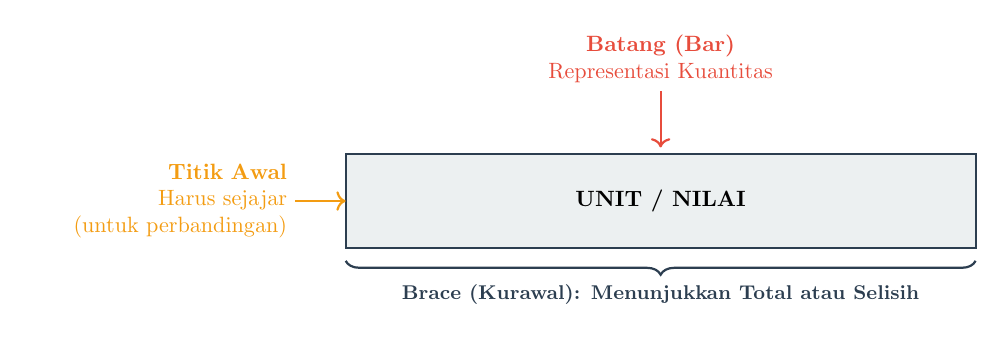
\begin{tikzpicture}[scale=0.8, transform shape]
        % Main Bar
        \draw[fill=softBgA, draw=mainBlue, thick] (0,0) rectangle (10, 1.5);
        
        % Labels inside
        \node at (5, 0.75) {\textbf{UNIT / NILAI}};
        
        % Anatomy annotations
        \draw[<-, thick, alertRed] (5, 1.6) -- (5, 2.5) node[above, align=center] {\textbf{Batang (Bar)}\\Representasi Kuantitas};
        \draw[<-, thick, niceOrange] (0, 0.75) -- (-0.8, 0.75) node[left, align=right, text width=4cm] {\textbf{Titik Awal}\\Harus sejajar\\(untuk perbandingan)};
        
        % Brace
        \DrawBraceDown{0}{10}{-0.2}{Brace (Kurawal): Menunjukkan Total atau Selisih}
    \end{tikzpicture}
    \vspace{0.2cm} \hrule \vspace{0.2cm}
    \begin{minipage}{0.9\textwidth}
        \textbf{Prinsip Dasar:}
        \begin{itemize}[leftmargin=*, label=\checkbox]
            \item \textbf{Panjang Proporsional:} Nilai yang lebih besar digambar lebih panjang (sketsa, tidak perlu presisi milimeter).
            \item \textbf{Konservasi:} Batang bisa dipotong, digeser, atau digabung tanpa mengubah nilai totalnya.
        \end{itemize}
    \end{minipage}
\end{tcolorbox}

% --- SECTION 3: C-P-A BRIDGE ---
\begin{tcolorbox}[title=\textbf{3. TRANSISI C-P-A (PENGENALAN ALJABAR)}, colback=softBgA, colframe=niceOrange, coltitle=white, fonttitle=\bfseries\large]
    \centering
    \begin{tikzpicture}[node distance=0.2cm and 0.5cm]
        \node[conceptBox] (concrete) {
            \textbf{A. KONKRET}\\ \textit{3 Keranjang "x"}\\ \vspace{0.1cm}
            \begin{tikzpicture}[scale=0.4, baseline=0] 
                % Basket 1
                \begin{scope}[shift={(0,0)}]
                    \draw[thick, mainBlue] (0.1,0.2) to[out=110, in=70] (1.4,0.2);
                    \draw[fill=niceOrange!40, draw=mainBlue, thick] (0,0.2) -- (0.25,-0.6) -- (1.25,-0.6) -- (1.5,0.2) -- cycle;
                    \node[font=\bfseries\large, mainBlue] at (0.75, -0.2) {$x$};
                \end{scope}
                % Basket 2
                \begin{scope}[shift={(1.8,0)}]
                    \draw[thick, mainBlue] (0.1,0.2) to[out=110, in=70] (1.4,0.2);
                    \draw[fill=niceOrange!40, draw=mainBlue, thick] (0,0.2) -- (0.25,-0.6) -- (1.25,-0.6) -- (1.5,0.2) -- cycle;
                    \node[font=\bfseries\large, mainBlue] at (0.75, -0.2) {$x$};
                \end{scope}
                % Basket 3
                \begin{scope}[shift={(3.6,0)}]
                    \draw[thick, mainBlue] (0.1,0.2) to[out=110, in=70] (1.4,0.2);
                    \draw[fill=niceOrange!40, draw=mainBlue, thick] (0,0.2) -- (0.25,-0.6) -- (1.25,-0.6) -- (1.5,0.2) -- cycle;
                    \node[font=\bfseries\large, mainBlue] at (0.75, -0.2) {$x$};
                \end{scope}
            \end{tikzpicture}
        };
        \node[conceptBox, right=of concrete] (pictorial) {
            \textbf{B. PIKTORIAL}\\ \textit{3 Himpunan Variabel}\\ \vspace{0.1cm}
            
\begin{tikzpicture}[scale=0.5, baseline=-5] 
                % Circle 1
                \draw[thick, mainBlue, fill=white] (0, 0) circle (0.6);
                \node[font=\bfseries\large, mainBlue, anchor=center] at (0, 0) {$x$};
                
                % Circle 2
                \draw[thick, mainBlue, fill=white] (1.5, 0) circle (0.6);
                \node[font=\bfseries\large, mainBlue, anchor=center] at (1.5, 0) {$x$};
                
                % Circle 3
                \draw[thick, mainBlue, fill=white] (3.0, 0) circle (0.6);
                \node[font=\bfseries\large, mainBlue, anchor=center] at (3.0, 0) {$x$};
            \end{tikzpicture}
        };
        \node[conceptBox, right=of pictorial] (abstract) {
            \textbf{C. ABSTRAK}\\ \textit{Aljabar}\\ \vspace{0.1cm}
            \tikz{\node[font=\bfseries\Huge, color=mainBlue] {3x};}
        };
        \draw[arrowFlow] (concrete) -- (pictorial); 
        \draw[arrowFlow] (pictorial) -- (abstract);
    \end{tikzpicture}
\end{tcolorbox}

\newpage

% --- EMPAT LOGIKA UTAMA ---
\begin{tcolorbox}[colback=mainBlue, colframe=mainBlue, arc=0mm, boxrule=0pt, top=4mm, bottom=4mm, halign=center]
    {\Huge \bfseries \color{white} STRUKTUR DASAR} \\
    \vspace{0.1cm}
    {\large \color{accentTeal} \textbf{Empat Logika Utama Bar Model}}
\end{tcolorbox}
\vspace{0.3cm}

% --- TYPE 1: PART-WHOLE ---
\begin{ConceptBox}{TIPE 1: PART-WHOLE MODEL (Bagian-Keseluruhan)}
\begin{minipage}{0.45\textwidth}
    \centering
    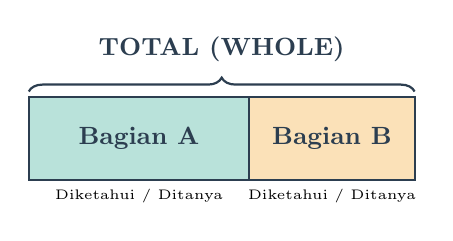
\begin{tikzpicture}[scale=0.7]
        % Whole Bar split into two
        \draw[fill=accentTeal!30, draw=mainBlue, thick] (0,0) rectangle (4, 1.5);
        \draw[fill=niceOrange!30, draw=mainBlue, thick] (4,0) rectangle (7, 1.5);
        
        % Labels
        \node[modelLabel] at (2, 0.75) {Bagian A};
        \node[modelLabel] at (5.5, 0.75) {Bagian B};
        
        % Braces
        \DrawBraceUp{0}{7}{1.6}{TOTAL (WHOLE)}
        \node[font=\tiny, below] at (2,0) {Diketahui / Ditanya};
        \node[font=\tiny, below] at (5.5,0) {Diketahui / Ditanya};
    \end{tikzpicture}
\end{minipage}%
\hfill
\begin{minipage}{0.5\textwidth}
    \textbf{Kapan Digunakan?}
    \begin{itemize}[leftmargin=*, itemsep=2pt]
        \item Operasi Penjumlahan (Mencari Total).
        \item Operasi Pengurangan (Diketahui Total dan satu Bagian, mencari Bagian lain).
        \item Tidak ada perbandingan "lebih banyak/sedikit".
    \end{itemize}
    \textit{Contoh Kalimat: "A dan B digabungkan...", "Sebagian adalah A, sisanya B..."}
\end{minipage}
\end{ConceptBox}

\vspace{0.3cm}

% --- TYPE 2: COMPARISON ---
\begin{ConceptBox}{TIPE 2: COMPARISON MODEL (Perbandingan)}
\begin{minipage}{0.45\textwidth}
    \centering
    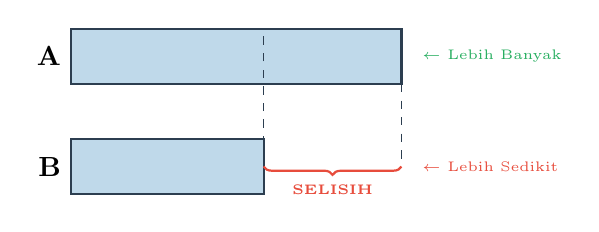
\begin{tikzpicture}[scale=0.7]
        % Bar A
        \node[left, font=\bfseries] at (0, 2.5) {A};
        \draw[fill=powerBlue!30, draw=mainBlue, thick] (0,2) rectangle (6, 3);
        
        % Bar B (Shorter)
        \node[left, font=\bfseries] at (0, 0.5) {B};
        \draw[fill=powerBlue!30, draw=mainBlue, thick] (0,0) rectangle (3.5, 1);
        
        % Dotted lines for comparison
        \draw[dashed, mainBlue] (3.5, 0) -- (3.5, 3);
        \draw[dashed, mainBlue] (6, 2) -- (6, 0.5);
        
        % Difference Brace
        \draw[decorate, decoration={brace, mirror, amplitude=3pt}, thick, alertRed] (3.5, 0.5) -- (6, 0.5) node[midway, below=3pt, font=\bfseries\tiny] {SELISIH};
        
        % Comparison logic - MOVED TO THE RIGHT TO AVOID COLLISION
        \node[font=\tiny, anchor=west, text=solGreen] at (6.2, 2.5) {$\leftarrow$ Lebih Banyak};
        \node[font=\tiny, anchor=west, text=alertRed] at (6.2, 0.5) {$\leftarrow$ Lebih Sedikit};
    \end{tikzpicture}
\end{minipage}%
\hfill
\begin{minipage}{0.5\textwidth}
    \textbf{Kapan Digunakan?}
    \begin{itemize}[leftmargin=*, itemsep=2pt]
        \item Membandingkan dua entitas berbeda.
        \item Kata kunci: "Lebih banyak dari", "Lebih sedikit dari", "Berapa bedanya", "Sama banyak dengan".
    \end{itemize}
    \textbf{Konsep Kunci:} Alignment (Kesejajaran) di sisi kiri sangat krusial untuk melihat selisih di sisi kanan.
\end{minipage}
\end{ConceptBox}

\vspace{0.3cm}

% --- TYPE 3: EQUAL PARTS / MULTIPLICATION ---
\begin{ConceptBox}{TIPE 3: EQUAL PARTS (Perkalian \& Pembagian)}
\begin{minipage}{0.45\textwidth}
    \centering
    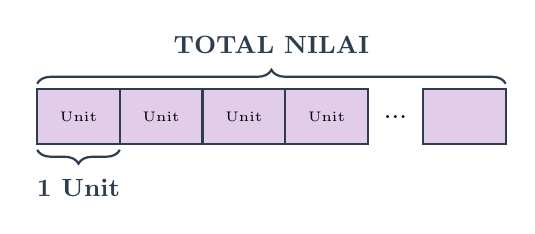
\begin{tikzpicture}[scale=0.7]
        % Bar split into equal parts
        \foreach \x in {0, 1.5, 3, 4.5} {
            \draw[fill=lightPurple!30, draw=mainBlue, thick] (\x, 0) rectangle (\x+1.5, 1);
            \node[font=\tiny] at (\x+0.75, 0.5) {Unit};
        }
        
        % Dot dot dot implies many
        \node at (6.5, 0.5) {...};
        \draw[fill=lightPurple!30, draw=mainBlue, thick] (7, 0) rectangle (8.5, 1);
        
        % Braces
        \DrawBraceDown{0}{1.5}{-0.1}{1 Unit}
        \DrawBraceUp{0}{8.5}{1.1}{TOTAL NILAI}
        
    \end{tikzpicture}
\end{minipage}%
\hfill
\begin{minipage}{0.5\textwidth}
    \textbf{Kapan Digunakan?}
    \begin{itemize}[leftmargin=*, itemsep=2pt]
        \item Benda-benda identik dalam jumlah banyak.
        \item Pecahan (Fraction): 1 bagian dari 5 bagian yang sama.
        \item Rasio (Perbandingan Senilai): 3 kotak vs 2 kotak.
    \end{itemize}
    \textbf{Konsep Kunci:} "Unitary Method". Mencari nilai \textbf{1 Unit} adalah kunci untuk memecahkan seluruh masalah.
\end{minipage}
\end{ConceptBox}

\vspace{0.3cm}

% --- TYPE 4: BEFORE-AFTER / CHANGE ---
\begin{ConceptBox}{TIPE 4: CHANGE MODEL (Perubahan/Transformasi)}
\begin{minipage}{0.45\textwidth}
    \centering
    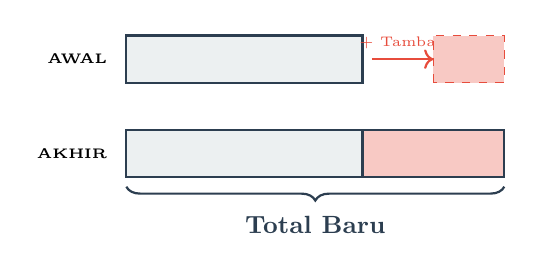
\begin{tikzpicture}[scale=0.6]
        % Before
        \node[anchor=east, font=\bfseries\tiny] at (-0.2, 2.5) {AWAL};
        \draw[fill=softBgA, draw=mainBlue, thick] (0,2) rectangle (5, 3);
        
        % Operation Arrow
        \draw[->, thick, alertRed] (5.2, 2.5) -- (6.5, 2.5) node[midway, above, font=\tiny] {+ Tambah};
        \draw[fill=alertRed!30, draw=alertRed, dashed] (6.5, 2) rectangle (8, 3);
        
        % After
        \node[anchor=east, font=\bfseries\tiny] at (-0.2, 0.5) {AKHIR};
        \draw[fill=softBgA, draw=mainBlue, thick] (0,0) rectangle (5, 1);
        \draw[fill=alertRed!30, draw=mainBlue, thick] (5,0) rectangle (8, 1);
        
        % Brace showing new total
        \DrawBraceDown{0}{8}{-0.2}{Total Baru}
    \end{tikzpicture}
\end{minipage}%
\hfill
\begin{minipage}{0.5\textwidth}
    \textbf{Kapan Digunakan?}
    \begin{itemize}[leftmargin=*, itemsep=2pt]
        \item Situasi dinamis (ada aksi).
        \item "Memberi", "Menerima", "Menjual", "Memakan".
    \end{itemize}
    \textbf{Konsep Kunci:} Visualisasikan proses penambahan (memperpanjang batang) atau pengurangan (memotong/mencoret batang).
\end{minipage}
\end{ConceptBox}

\newpage

% =================================================================================
% BAGIAN 2: SOAL 1-5
% =================================================================================
\part{LATIHAN SOAL (PAKET A: 1-5)}

\section*{Soal 1: Aljabar (Algebra)}

\textbf{Soal:}
Terdapat $x$ permen di dalam sebuah tas. Jane mengambil beberapa permen dari tas tersebut. Ruth mengambil dua kali lipat jumlah permen yang diambil Jane. Sally mengambil 25 permen lebih banyak daripada Jane. Tas tersebut sekarang kosong.
\begin{enumerate}[label=(\alph*)]
    \item Nyatakan jumlah permen yang diambil Jane dalam bentuk $x$.
    \item Jika $x = 265$, tentukan jumlah permen yang diambil oleh masing-masing anak.
\end{enumerate}

\hrulefill

\textbf{Pembahasan:}

Kita gambarkan setiap unit sebagai satu kotak utuh.

\begin{center}
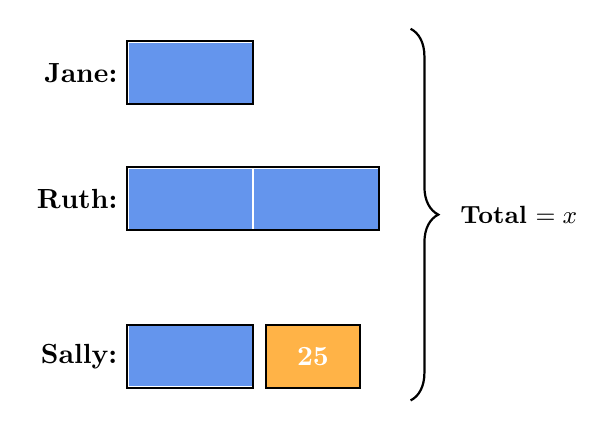
\begin{tikzpicture}[scale=0.8, every node/.style={font=\small}]
    % Jane: 1 kotak
    \node[anchor=east, font=\bfseries] at (0, 3) {Jane:};
    \draw[fill=colP, draw=white, line width=1pt] (0, 2.5) rectangle (2, 3.5);
    \draw[thick] (0, 2.5) rectangle (2, 3.5); % Border luar
    \node[white, font=\bfseries] at (1, 3) {};
    
    % Ruth: 2 kotak
    \node[anchor=east, font=\bfseries] at (0, 1) {Ruth:};
    \foreach \x in {0, 2} {
        \draw[fill=colP, draw=white, line width=1pt] (\x, 0.5) rectangle (\x+2, 1.5);
    }
    \draw[thick] (0, 0.5) rectangle (4, 1.5); % Border luar
    \node[white, font=\bfseries] at (1, 1) {};
    \node[white, font=\bfseries] at (3, 1) {};
    
    % Sally: 1 kotak + 25
    \node[anchor=east, font=\bfseries] at (0, -1.5) {Sally:};
    \draw[fill=colP, draw=white, line width=1pt] (0, -2) rectangle (2, -1);
    \draw[thick] (0, -2) rectangle (2, -1);
    \node[white, font=\bfseries] at (1, -1.5) {};
    
    % Bagian +25 (beda warna/ukuran)
    \draw[fill=colQ, draw=black, thick] (2.2, -2) rectangle (3.7, -1) node[midway, white, font=\bfseries] {25};
    
    % Total Brace
    \draw[decorate,decoration={brace,amplitude=10pt,mirror},thick] (4.5, -2.2) -- (4.5, 3.7) node[midway, right=0.5cm, align=left] {\textbf{Total} $= x$};
\end{tikzpicture}
\end{center}

Terlihat total unit kotak biru ada 4 buah.
\[ x = 4 \text{ kotak} + 25 \]

\textbf{(a) Menyatakan Jane dalam $x$}
Karena Jane memiliki tepat 1 kotak (1 unit):
\begin{align*}
    4 \text{ unit} + 25 &= x \\
    4 \text{ unit} &= x - 25 \\
    1 \text{ unit} &= \frac{x - 25}{4}
\end{align*}
Jadi, permen Jane = $\boxed{\frac{x - 25}{4}}$.

\textbf{(b) Jika $x = 265$}
\begin{align*}
    4 \text{ unit} &= 265 - 25 \\
    4 \text{ unit} &= 240 \\
    1 \text{ unit} &= 60
\end{align*}

Maka:
\begin{itemize}
    \item \textbf{Jane} (1 unit) = \textbf{60}
    \item \textbf{Ruth} (2 unit) = $60 \times 2$ = \textbf{120}
    \item \textbf{Sally} (1 unit + 25) = $60 + 25$ = \textbf{85}
\end{itemize}

\newpage

\section*{Soal 2: Perbandingan (Ratio)}

\textbf{Soal:}
Kota P memiliki $\frac{2}{5}$ jumlah penduduk Kota Q. Perbandingan jumlah penduduk di Kota R terhadap Kota P adalah $4:7$. Kota Q memiliki 8100 penduduk lebih banyak daripada Kota R. Berapa jumlah penduduk di Kota R?

\hrulefill

\textbf{Pembahasan:}

Kita perlu menyamakan "ukuran kotak" (unit) untuk Kota P agar bisa membandingkan ketiga kota.
\begin{itemize}
    \item P : Q = 2 : 5 (Kalikan 7) $\rightarrow$ P : Q = 14 : 35
    \item R : P = 4 : 7 (Kalikan 2) $\rightarrow$ R : P = 8 : 14
\end{itemize}
Sekarang unit P sudah sama (14 unit).

\begin{center}
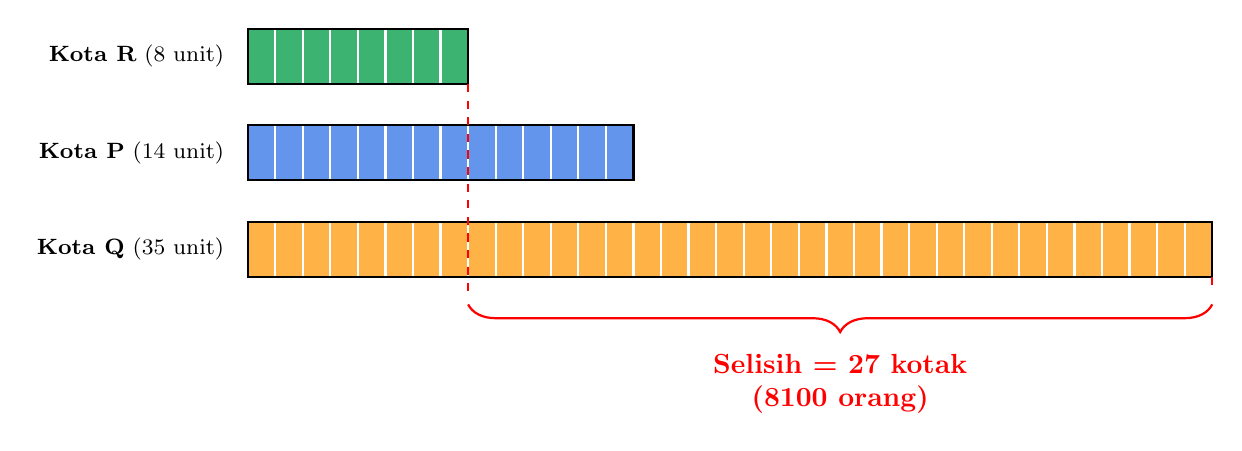
\begin{tikzpicture}[scale=0.35, every node/.style={font=\footnotesize}]
    % R (8 unit)
    \node[anchor=east] at (-0.5, 7) {\textbf{Kota R} (8 unit)};
    \draw[fill=colR] (0, 6) rectangle (8, 8);
    \foreach \x in {1,...,7} \draw[white, line width=0.8pt] (\x, 6) -- (\x, 8); % Grid lines
    \draw[thick] (0, 6) rectangle (8, 8); % Border
    
    % P (14 unit)
    \node[anchor=east] at (-0.5, 3.5) {\textbf{Kota P} (14 unit)};
    \draw[fill=colP] (0, 2.5) rectangle (14, 4.5);
    \foreach \x in {1,...,13} \draw[white, line width=0.8pt] (\x, 2.5) -- (\x, 4.5); % Grid lines
    \draw[thick] (0, 2.5) rectangle (14, 4.5); % Border
    
    % Q (35 unit)
    \node[anchor=east] at (-0.5, 0) {\textbf{Kota Q} (35 unit)};
    \draw[fill=colQ] (0, -1) rectangle (35, 1);
    \foreach \x in {1,...,34} \draw[white, line width=0.8pt] (\x, -1) -- (\x, 1); % Grid lines
    \draw[thick] (0, -1) rectangle (35, 1); % Border
    
    % Garis putus-putus penanda selisih
    \draw[dashed, red, thick] (8, 6) -- (8, -1.5);
    \draw[dashed, red, thick] (35, -1) -- (35, -1.5);
    
    % Brace Selisih
    \draw[decorate,decoration={brace,amplitude=10pt,mirror},thick, red] (8, -2) -- (35, -2) 
    node[midway, below=0.5cm, align=center, font=\bfseries, color=red] {Selisih = 27 kotak\\(8100 orang)};
\end{tikzpicture}
\end{center}

Dari gambar grid di atas:
Selisih panjang batang Q dan R adalah $35 - 8 = 27$ kotak.

\[ 27 \text{ unit} = 8100 \implies 1 \text{ unit} = 300 \]

\textbf{Kota R (8 unit):}
\[ 8 \times 300 = \mathbf{2.400} \text{ penduduk} \]

\newpage

\section*{Soal 3: Kecepatan (Speed)}

\textbf{Soal:}
Nathaniel dan Trevor masing-masing lari santai (joging) dari Taman E ke Taman F. Nathaniel membutuhkan waktu 2 jam untuk menempuh seluruh perjalanan, sedangkan Trevor membutuhkan waktu 1 jam untuk menempuh tiga perlima perjalanan tersebut. Tentukan rasio kecepatan rata-rata Nathaniel terhadap kecepatan rata-rata Trevor.

\hrulefill

\textbf{Pembahasan:}

Kita bandingkan \textbf{jarak yang ditempuh dalam waktu yang sama}, yaitu 1 jam.
Kita anggap Jarak Total = 10 unit jarak (KPK dari 2 dan 5 untuk mempermudah visualisasi).

\begin{center}
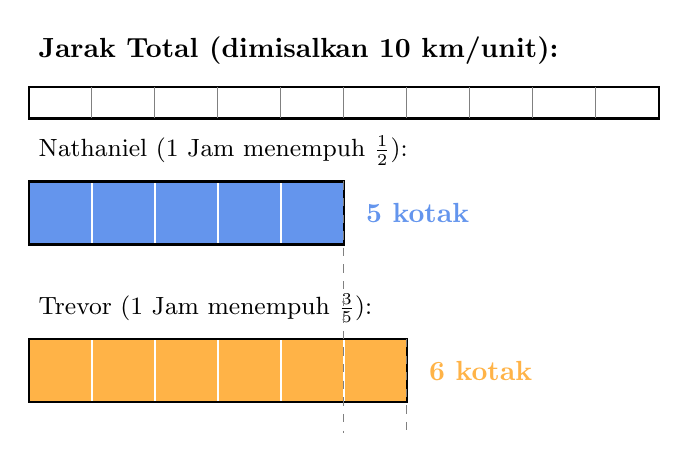
\begin{tikzpicture}[scale=0.8, every node/.style={font=\small}]
    % --- Header Jarak Total ---
    \node[anchor=south west, font=\bfseries] at (0, 6.2) {Jarak Total (dimisalkan 10 km/unit):};
    % Kotak Jarak Total (Kosong/Grid)
    \draw[thick] (0, 5.5) rectangle (10, 6);
    \foreach \x in {1,...,9} \draw[gray] (\x, 5.5) -- (\x, 6);
    
    % --- Nathaniel ---
    \node[anchor=south west] at (0, 4.6) {Nathaniel (1 Jam menempuh $\frac{1}{2}$):};
    % Batang Nathaniel (5 kotak)
    \draw[fill=colP] (0, 3.5) rectangle (5, 4.5);
    \foreach \x in {1,...,4} \draw[white, line width=0.8pt] (\x, 3.5) -- (\x, 4.5);
    \draw[thick] (0, 3.5) rectangle (5, 4.5); % Border
    % Label Jumlah Kotak
    \node[right, colP, font=\bfseries] at (5.2, 4) {5 kotak};

    % --- Trevor ---
    \node[anchor=south west] at (0, 2.1) {Trevor (1 Jam menempuh $\frac{3}{5}$):};
    % Batang Trevor (6 kotak)
    \draw[fill=colQ] (0, 1) rectangle (6, 2);
    \foreach \x in {1,...,5} \draw[white, line width=0.8pt] (\x, 1) -- (\x, 2);
    \draw[thick] (0, 1) rectangle (6, 2); % Border
    % Label Jumlah Kotak
    \node[right, colQ, font=\bfseries] at (6.2, 1.5) {6 kotak};
    
    % --- Garis Bantu ---
    \draw[dashed, gray] (5, 4.5) -- (5, 0.5); % Garis batas Nathaniel
    \draw[dashed, gray] (6, 2) -- (6, 0.5);    % Garis batas Trevor
\end{tikzpicture}
\end{center}

Rasio Kecepatan = Rasio Jarak (dalam 1 jam)
\[ \text{Nathaniel} : \text{Trevor} = 5 \text{ kotak} : 6 \text{ kotak} = \mathbf{5 : 6} \]

\newpage

\section*{Soal 4: Rasio Bertingkat (Ratio)}

\textbf{Soal:}
Rasio jumlah buku Claude terhadap buku Robin adalah $5:6$. Rasio jumlah buku Robin terhadap buku Ian adalah $7:4$. Jika Claude memiliki 22 buku lebih banyak daripada Ian, berapa banyak buku yang dimiliki Robin?

\hrulefill

\textbf{Pembahasan:}

Variabel penghubung adalah **Robin**. Kita harus menyamakan unit Robin pada kedua rasio.
\begin{itemize}
    \item C : R = 5 : 6 (Kalikan 7) $\rightarrow$ \textbf{35 : 42}
    \item R : I = 7 : 4 (Kalikan 6) $\rightarrow$ \textbf{42 : 24}
\end{itemize}
Rasio gabungan C : R : I = 35 : 42 : 24.

\begin{center}
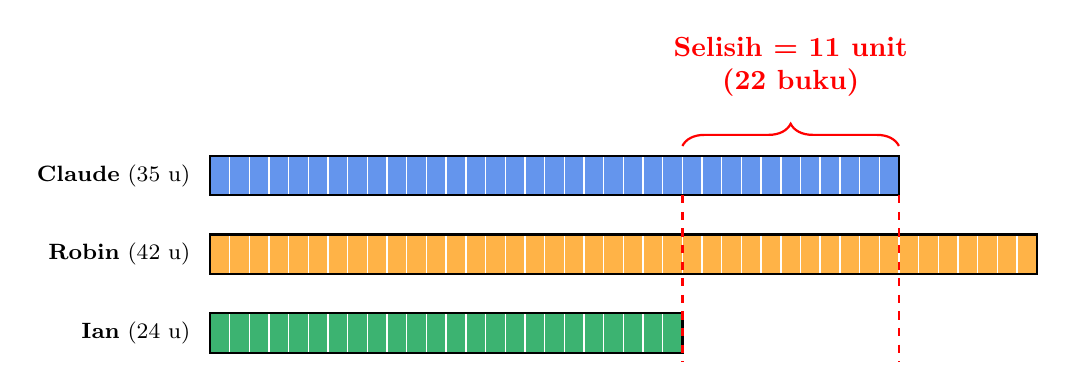
\begin{tikzpicture}[scale=0.25, every node/.style={font=\footnotesize}]
    % Claude (35 unit)
    \node[anchor=east] at (-0.5, 8) {\textbf{Claude} (35 u)};
    \draw[fill=colP] (0, 7) rectangle (35, 9);
    \foreach \x in {1,...,34} \draw[white, line width=0.5pt] (\x, 7) -- (\x, 9); % Grid halus
    \draw[thick] (0, 7) rectangle (35, 9);
    
    % Robin (42 unit)
    \node[anchor=east] at (-0.5, 4) {\textbf{Robin} (42 u)};
    \draw[fill=colQ] (0, 3) rectangle (42, 5);
    \foreach \x in {1,...,41} \draw[white, line width=0.5pt] (\x, 3) -- (\x, 5);
    \draw[thick] (0, 3) rectangle (42, 5);
    
    % Ian (24 unit)
    \node[anchor=east] at (-0.5, 0) {\textbf{Ian} (24 u)};
    \draw[fill=colR] (0, -1) rectangle (24, 1);
    \foreach \x in {1,...,23} \draw[white, line width=0.5pt] (\x, -1) -- (\x, 1);
    \draw[thick] (0, -1) rectangle (24, 1);
    
    % Penanda Selisih
    \draw[dashed, red, thick] (24, 7) -- (24, -1.5);
    \draw[dashed, red, thick] (35, 7) -- (35, -1.5);
    
    \draw[decorate,decoration={brace,amplitude=8pt},thick, red] (24, 9.5) -- (35, 9.5) 
    node[midway, above=0.5cm, align=center, font=\bfseries, color=red] {Selisih = 11 unit\\(22 buku)};
\end{tikzpicture}
\end{center}

Selisih unit Claude dan Ian: $35 - 24 = 11$ unit.
\[ 11 \text{ unit} = 22 \text{ buku} \implies 1 \text{ unit} = 2 \text{ buku} \]

\textbf{Jumlah buku Robin (42 unit):}
\[ 42 \times 2 = \mathbf{84} \text{ buku} \]

\newpage

\section*{Soal 5: Pecahan Sisa (Fraction of Remainder)}

\textbf{Soal:}
Gavin memiliki sejumlah uang. Ia menyumbangkan $\frac{1}{2}$ dari uangnya ke Yayasan A. Kemudian, ia menyumbangkan $\frac{1}{4}$ dari sisanya ke Palang Merah. Selanjutnya, ia memberikan $\frac{1}{3}$ dari sisanya lagi ke Mercy Corps. Terakhir, ia mendonasikan $\frac{1}{2}$ dari sisanya ke Global Fund. Gavin tersisa \$625 pada akhirnya. Berapa uang Gavin mula-mula?

\hrulefill

\textbf{Pembahasan (Working Backwards):}

Kita gambar kotaknya secara harfiah untuk melihat sisa dengan metode mundur.

\begin{center}
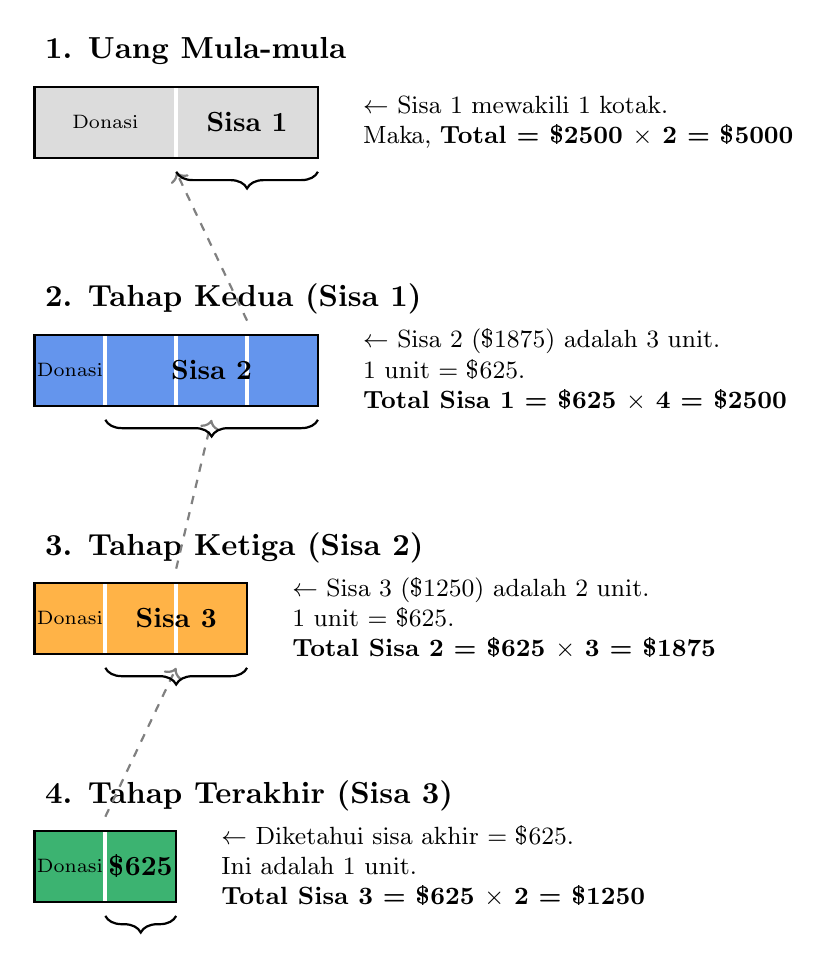
\begin{tikzpicture}[scale=0.9, every node/.style={font=\small}]
    % --- Bar 4: Sisa 3 ---
    \node[anchor=west, font=\bfseries, scale=1.1] at (0, 1.5) {4. Tahap Terakhir (Sisa 3)};
    % Sisa akhir 1/2 bagian. Kita gambar Sisa 3 sebagai 2 kotak.
    \draw[fill=colR] (0, 0) rectangle (2, 1);
    \draw[white, line width=1.5pt] (1, 0) -- (1, 1);
    \draw[thick] (0, 0) rectangle (2, 1);
    
    \node at (0.5, 0.5) {\scriptsize Donasi};
    \node[font=\bfseries] at (1.5, 0.5) {\$625};
    
    % Brace Sisa Akhir
    \draw[decorate,decoration={brace,amplitude=6pt,mirror},thick] (1, -0.2) -- (2, -0.2);
    
    % Penjelasan Kanan
    \node[right, align=left] at (2.5, 0.5) {
        $\leftarrow$ Diketahui sisa akhir = \$625.\\
        Ini adalah 1 unit.\\
        \textbf{Total Sisa 3 = \$625 $\times$ 2 = \$1250}
    };

    % Panah penghubung ke atas
    \draw[dashed, ->, thick, gray] (1, 1.2) -- (2, 3.3);

    % --- Bar 3: Sisa 2 ---
    \node[anchor=west, font=\bfseries, scale=1.1] at (0, 5) {3. Tahap Ketiga (Sisa 2)};
    % Sisa 3 mewakili 2/3 bagian (karena 1/3 didonasikan).
    % Kita gambar Sisa 2 sebagai 3 kotak.
    \draw[fill=colQ] (0, 3.5) rectangle (3, 4.5);
    \foreach \x in {1,2} \draw[white, line width=1.5pt] (\x, 3.5) -- (\x, 4.5);
    \draw[thick] (0, 3.5) rectangle (3, 4.5);
    
    \node at (0.5, 4) {\scriptsize Donasi};
    \node[font=\bfseries] at (2, 4) {Sisa 3};
    
    % Brace Sisa 3 (Mencakup 2 kotak kanan)
    \draw[decorate,decoration={brace,amplitude=6pt,mirror},thick] (1, 3.3) -- (3, 3.3);
    
    % Penjelasan Kanan
    \node[right, align=left] at (3.5, 4) {
        $\leftarrow$ Sisa 3 (\$1250) adalah 2 unit.\\
        1 unit = \$625.\\
        \textbf{Total Sisa 2 = \$625 $\times$ 3 = \$1875}
    };

    % Panah penghubung ke atas
    \draw[dashed, ->, thick, gray] (2, 4.7) -- (2.5, 6.8);

    % --- Bar 2: Sisa 1 ---
    \node[anchor=west, font=\bfseries, scale=1.1] at (0, 8.5) {2. Tahap Kedua (Sisa 1)};
    % Sisa 2 mewakili 3/4 bagian (karena 1/4 didonasikan).
    % Kita gambar Sisa 1 sebagai 4 kotak.
    \draw[fill=colP] (0, 7) rectangle (4, 8);
    \foreach \x in {1,2,3} \draw[white, line width=1.5pt] (\x, 7) -- (\x, 8);
    \draw[thick] (0, 7) rectangle (4, 8);
    
    \node at (0.5, 7.5) {\scriptsize Donasi};
    \node[font=\bfseries] at (2.5, 7.5) {Sisa 2};
    
    % Brace Sisa 2 (Mencakup 3 kotak kanan)
    \draw[decorate,decoration={brace,amplitude=6pt,mirror},thick] (1, 6.8) -- (4, 6.8);
    
    % Penjelasan Kanan
    \node[right, align=left] at (4.5, 7.5) {
        $\leftarrow$ Sisa 2 (\$1875) adalah 3 unit.\\
        1 unit = \$625.\\
        \textbf{Total Sisa 1 = \$625 $\times$ 4 = \$2500}
    };

    % Panah penghubung ke atas
    \draw[dashed, ->, thick, gray] (3, 8.2) -- (2, 10.3);

    % --- Bar 1: Mula-mula ---
    \node[anchor=west, font=\bfseries, scale=1.1] at (0, 12) {1. Uang Mula-mula};
    % Sisa 1 mewakili 1/2 bagian (karena 1/2 didonasikan). 
    % Artinya Mula-mula = 2 kotak.
    \draw[fill=colGrayMid, draw=black] (0, 10.5) rectangle (4, 11.5);
    \draw[white, line width=1.5pt] (2, 10.5) -- (2, 11.5);
    \draw[thick] (0, 10.5) rectangle (4, 11.5);
    
    \node at (1, 11) {\scriptsize Donasi};
    \node[font=\bfseries] at (3, 11) {Sisa 1};
    
    % Brace Sisa 1
    \draw[decorate,decoration={brace,amplitude=6pt,mirror},thick] (2, 10.3) -- (4, 10.3);
    
    % Penjelasan Kanan
    \node[right, align=left] at (4.5, 11) {
        $\leftarrow$ Sisa 1 mewakili 1 kotak.\\
        Maka, \textbf{Total = \$2500 $\times$ 2 = \$5000}
    };

\end{tikzpicture}
\end{center}

Jadi, uang Gavin mula-mula adalah \textbf{\$5.000}.

\newpage

% =================================================================================
% BAGIAN 3: SOAL 6-10 (Lanjutan)
% =================================================================================
\part{LATIHAN SOAL (PAKET B: 6-10)}

\section*{Soal 6: Bilangan Cacah (Quotient \& Remainder)}
\textbf{Soal:}
Ketika Bilangan X dibagi dengan Bilangan Y, hasil baginya adalah 16 dan sisanya 3. Jumlah dari kedua bilangan, hasil bagi, dan sisanya adalah 345. Berapakah Bilangan X?

\hrulefill

\textbf{Pembahasan:}

Dari soal, kita tahu hubungan: $X = (16 \times Y) + 3$.
Jika kita gambarkan dalam kotak unit:
\begin{itemize}
    \item \textbf{Bilangan Y} = 1 kotak unit.
    \item \textbf{Bilangan X} = 16 kotak unit + nilai 3.
\end{itemize}

Persamaan totalnya:
\[ X + Y + 16 + 3 = 345 \]
\[ (16 \text{ unit} + 3) + (1 \text{ unit}) + 19 = 345 \]
\[ 17 \text{ unit} + 22 = 345 \]
\[ 17 \text{ unit} = 323 \]

\vspace{0.5cm}
\begin{center}
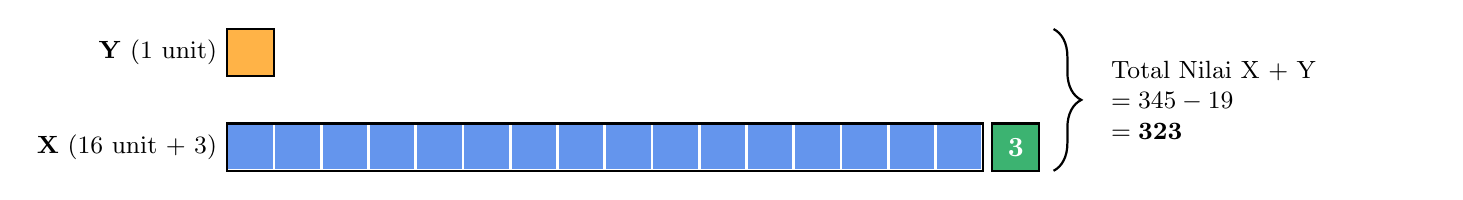
\begin{tikzpicture}[scale=0.6, every node/.style={font=\small}]
    % --- Bar Y ---
    \node[anchor=east] at (0, 3) {\textbf{Y} (1 unit)};
    \draw[fill=colOrange, draw=white, line width=1pt] (0, 2.5) rectangle (1, 3.5);
    \draw[thick] (0, 2.5) rectangle (1, 3.5); % Border
    \node at (0.5, 3) {};

    % --- Bar X ---
    \node[anchor=east] at (0, 1) {\textbf{X} (16 unit + 3)};
    % Loop menggambar 16 kotak biru
    \foreach \x in {0, ..., 15} {
        \draw[fill=colBlue, draw=white, line width=1pt] (\x, 0.5) rectangle (\x+1, 1.5);
    }
    \draw[thick] (0, 0.5) rectangle (16, 1.5); % Border luar unit
    
    % Kotak sisa 3 (Beda warna & ukuran fix visual)
    \draw[fill=colGreen, draw=black, thick] (16.2, 0.5) rectangle (17.2, 1.5);
    \node[white, font=\bfseries] at (16.7, 1) {3};

    % Label Unit
    \node[white] at (0.5, 1) {};
    \node[white] at (15.5, 1) {};
    \node at (8, 1) {};

    % Brace Total
    \draw[decorate,decoration={brace,amplitude=10pt,mirror},thick] (17.5, 0.5) -- (17.5, 3.5) 
    node[midway, right=0.6cm, align=left, text width=4cm] {Total Nilai X + Y\\$= 345 - 19$\\$= \mathbf{323}$};
\end{tikzpicture}
\end{center}
\vspace{0.5cm}

\textbf{Hitungan:}
\[ 1 \text{ unit} = 323 \div 17 = 19 \quad (\text{Nilai Y}) \]
\[ X = (16 \times 19) + 3 = 304 + 3 = \mathbf{307} \]

\newpage

\section*{Soal 7: Pecahan (Equal Fractions)}
\textbf{Soal:}
Di Peternakan A, $\frac{4}{5}$ dari jumlah domba sama dengan $\frac{1}{2}$ dari jumlah domba di Peternakan B. Total domba di Peternakan A dan Peternakan B adalah 845 ekor. Berapa jumlah domba di Peternakan B?

\hrulefill

\textbf{Pembahasan:}

Samakan pembilang pecahan agar unit pembandingnya setara (Equal Units).
\begin{itemize}
    \item Peternakan A: $\frac{4}{5}$ (4 kotak dari total 5).
    \item Peternakan B: $\frac{1}{2} = \frac{4}{8}$ (4 kotak dari total 8).
\end{itemize}
Jadi, kita gambar 4 kotak yang "sama besar" untuk kedua peternakan sebagai jembatan.

\vspace{0.5cm}
\begin{center}
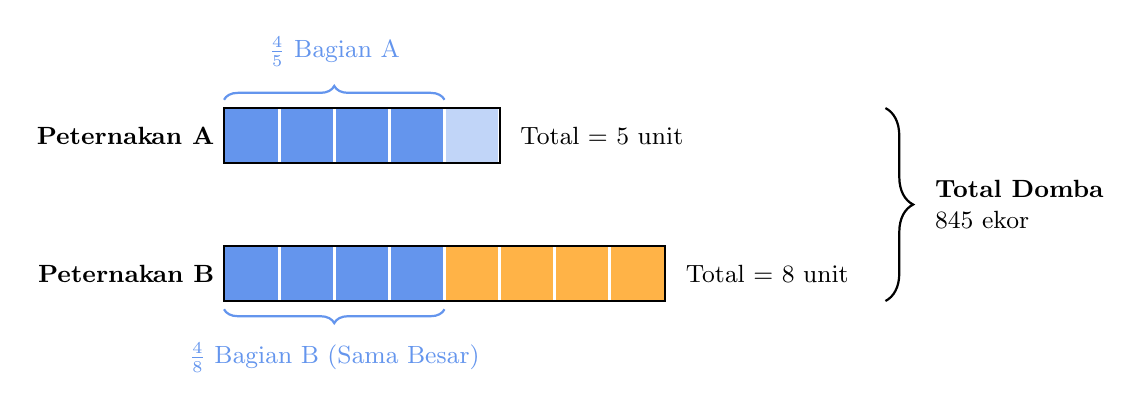
\begin{tikzpicture}[scale=0.7, every node/.style={font=\small}]
    % --- Peternakan A ---
    \node[anchor=east] at (0, 4) {\textbf{Peternakan A}};
    % 4 Unit Setara (Biru)
    \foreach \x in {0, ..., 3} {
        \draw[fill=colBlue, draw=white, line width=1pt] (\x, 3.5) rectangle (\x+1, 4.5);
    }
    % 1 Unit Sisa (Biru Muda - bagian dari total A)
    \draw[fill=colBlue!40, draw=white, line width=1pt] (4, 3.5) rectangle (5, 4.5);
    \draw[thick] (0, 3.5) rectangle (5, 4.5); % Border
    \node[right] at (5.2, 4) {Total = 5 unit};

    % --- Peternakan B ---
    \node[anchor=east] at (0, 1.5) {\textbf{Peternakan B}};
    % 4 Unit Setara (Biru) - Sejajar dengan atas
    \foreach \x in {0, ..., 3} {
        \draw[fill=colBlue, draw=white, line width=1pt] (\x, 1) rectangle (\x+1, 2);
    }
    % 4 Unit Sisa (Oranye - total B ada 8)
    \foreach \x in {4, ..., 7} {
        \draw[fill=colOrange, draw=white, line width=1pt] (\x, 1) rectangle (\x+1, 2);
    }
    \draw[thick] (0, 1) rectangle (8, 2); % Border
    \node[right] at (8.2, 1.5) {Total = 8 unit};

    % Brace Hubungan (Atas & Bawah)
    \draw[decorate,decoration={brace,amplitude=5pt,raise=3pt}, thick, color=colBlue] (0, 4.5) -- (4, 4.5) node[midway, above=0.4cm] {$\frac{4}{5}$ Bagian A};
    \draw[decorate,decoration={brace,amplitude=5pt,mirror,raise=3pt}, thick, color=colBlue] (0, 1) -- (4, 1) node[midway, below=0.4cm] {$\frac{4}{8}$ Bagian B (Sama Besar)};

    % Brace Total Keseluruhan (DI KANAN)
    % Menjangkau dari bawah B (y=1) sampai atas A (y=4.5)
    \draw[decorate,decoration={brace,amplitude=10pt,mirror}, thick] (12, 1) -- (12, 4.5) 
    node[midway, right=0.5cm, align=left] {\textbf{Total Domba}\\845 ekor};

\end{tikzpicture}
\end{center}
\vspace{0.5cm}

\textbf{Hitungan:}
Total seluruh kotak unit = 5 (A) + 8 (B) = 13 unit.
\[ 13 \text{ unit} = 845 \]
\[ 1 \text{ unit} = 845 \div 13 = 65 \text{ ekor} \]
Peternakan B memiliki 8 unit:
\[ 8 \times 65 = \mathbf{520} \text{ ekor} \]

\newpage

\section*{Soal 8: Rasio (Before and After)}
\textbf{Soal:}
Rasio uang Terry terhadap uang Maria awalnya adalah 4:9. Setelah Terry membelanjakan setengah uangnya dan Maria membelanjakan \$20, uang Maria menjadi dua kali lipat uang Terry. Berapa uang Terry mula-mula?

\hrulefill

\textbf{Pembahasan:}

Gunakan kotak unit untuk melacak perubahan.
\begin{itemize}
    \item \textbf{Awal:} Terry (4 kotak), Maria (9 kotak).
    \item \textbf{Aksi:} Terry sisa 2 kotak (karena setengahnya habis).
    \item \textbf{Syarat Akhir:} Uang Maria = 2 $\times$ Uang Terry. 
    Karena sisa Terry adalah 2 kotak, maka sisa Maria haruslah $2 \times 2 = \mathbf{4 \text{ kotak}}$.
\end{itemize}

\vspace{0.5cm}
\begin{center}
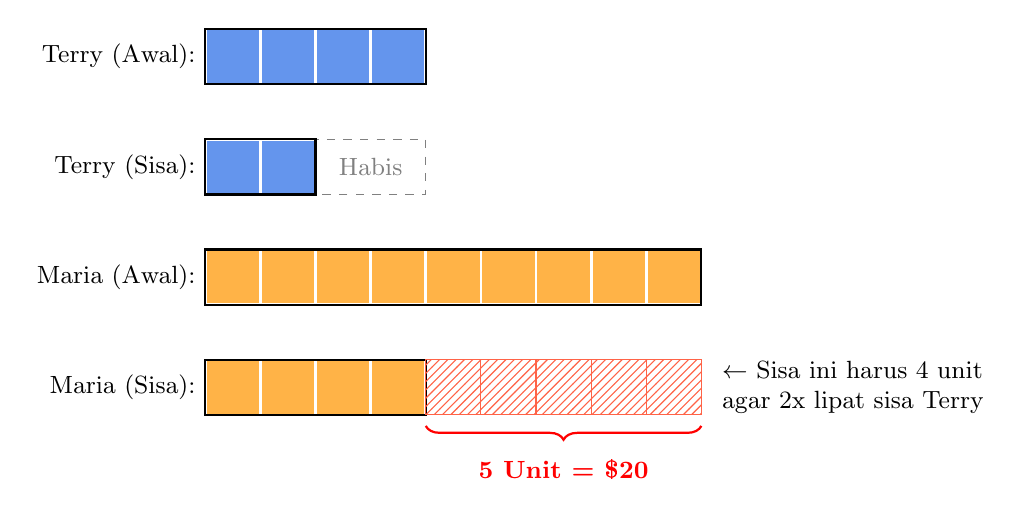
\begin{tikzpicture}[scale=0.7, every node/.style={font=\small}]
    % --- Terry Awal ---
    \node[anchor=east] at (0, 6) {Terry (Awal):};
    \foreach \x in {0, ..., 3} {
        \draw[fill=colBlue, draw=white, line width=1pt] (\x, 5.5) rectangle (\x+1, 6.5);
    }
    \draw[thick] (0, 5.5) rectangle (4, 6.5); 

    % --- Terry Akhir ---
    \node[anchor=east] at (0, 4) {Terry (Sisa):};
    % 2 Kotak Sisa
    \foreach \x in {0, 1} {
        \draw[fill=colBlue, draw=white, line width=1pt] (\x, 3.5) rectangle (\x+1, 4.5);
    }
    % 2 Kotak Hilang (Dashed)
    \draw[dashed, draw=gray] (2, 3.5) rectangle (4, 4.5);
    \node[gray] at (3, 4) {Habis};
    \draw[thick] (0, 3.5) rectangle (2, 4.5); % Border sisa

    % --- Maria Awal ---
    \node[anchor=east] at (0, 2) {Maria (Awal):};
    \foreach \x in {0, ..., 8} {
        \draw[fill=colOrange, draw=white, line width=1pt] (\x, 1.5) rectangle (\x+1, 2.5);
    }
    \draw[thick] (0, 1.5) rectangle (9, 2.5);

    % --- Maria Akhir ---
    \node[anchor=east] at (0, 0) {Maria (Sisa):};
    % 4 Kotak Sisa (Target)
    \foreach \x in {0, ..., 3} {
        \draw[fill=colOrange, draw=white, line width=1pt] (\x, -0.5) rectangle (\x+1, 0.5);
    }
    \draw[thick] (0, -0.5) rectangle (4, 0.5);
    
    % 5 Kotak Hilang ($20)
    \foreach \x in {4, ..., 8} {
        \draw[pattern=north east lines, pattern color=colRed, draw=colRed] (\x, -0.5) rectangle (\x+1, 0.5);
    }
    
    % Brace Penjelasan Logika
    \draw[decorate,decoration={brace,amplitude=5pt,mirror}, thick, red] (4, -0.7) -- (9, -0.7) 
    node[midway, below=0.3cm] {\textbf{5 Unit = \$20}};
    
    \node[right, align=left] at (9.2, 0) {$\leftarrow$ Sisa ini harus 4 unit\\agar 2x lipat sisa Terry};

\end{tikzpicture}
\end{center}
\vspace{0.5cm}

\textbf{Hitungan:}
Dari gambar Maria (Akhir), selisih kotak awal (9) dan kotak sisa (4) adalah 5 kotak.
5 kotak ini mewakili uang yang dibelanjakan (\$20).
\[ 5 \text{ kotak} = \$20 \implies 1 \text{ kotak} = \$4 \]
Uang Terry Mula-mula (4 kotak):
\[ 4 \times \$4 = \mathbf{\$16} \]

\newpage

\section*{Soal 9: Perbandingan Dua Skenario (Gap \& Difference)}
\textbf{Soal:}
Ryan dan Marie memiliki sejumlah kelereng. 
\begin{itemize}
    \item \textbf{Skenario 1:} Jika Ryan kehilangan 15 kelereng, rasionya Ryan:Marie = 4:1.
    \item \textbf{Skenario 2:} Jika Ryan kehilangan 75 kelereng, rasionya Ryan:Marie = 3:2.
\end{itemize}
Berapa banyak kelereng Ryan mula-mula?

\hrulefill

\textbf{Pembahasan:}

Jumlah kelereng Marie **TETAP**. Kita jadikan Marie sebagai patokan unit yang sama.
\begin{itemize}
    \item Skenario 1: Ryan : Marie = 4 : 1. (Ubah jadi \textbf{8 : 2} agar Marie sama dengan skenario 2).
    \item Skenario 2: Ryan : Marie = \textbf{3 : 2}.
\end{itemize}
Jadi, kita gunakan **2 kotak** untuk Marie di kedua gambar.

\vspace{0.5cm}
\begin{center}
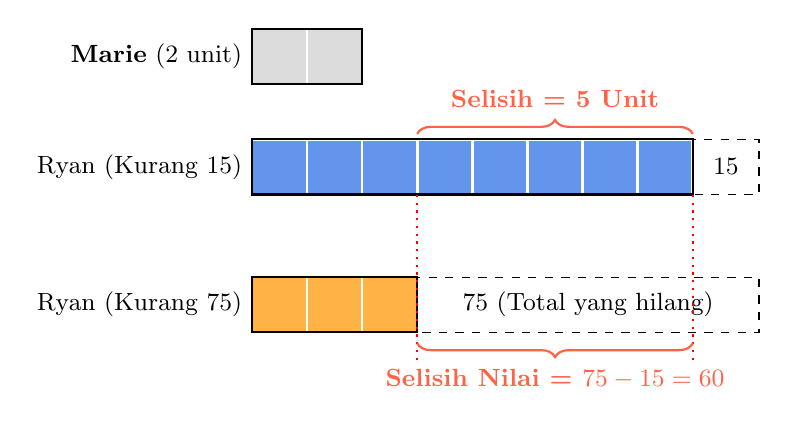
\begin{tikzpicture}[scale=0.7, every node/.style={font=\small}]
    % --- Marie (Konstan) ---
    \node[anchor=east] at (0, 6) {\textbf{Marie} (2 unit)};
    \foreach \x in {0, 1} {
        \draw[fill=colGray, draw=white, line width=1pt] (\x, 5.5) rectangle (\x+1, 6.5);
    }
    \draw[thick] (0, 5.5) rectangle (2, 6.5);

    % --- Ryan Skenario 1 ---
    \node[anchor=east] at (0, 4) {Ryan (Kurang 15)};
    % 8 Unit
    \foreach \x in {0, ..., 7} {
        \draw[fill=colBlue, draw=white, line width=1pt] (\x, 3.5) rectangle (\x+1, 4.5);
    }
    \draw[thick] (0, 3.5) rectangle (8, 4.5);
    % Kotak putus-putus +15 (Posisi relatif di kanan)
    \draw[dashed] (8, 3.5) rectangle (9.2, 4.5);
    \node at (8.6, 4) {15};

    % --- Ryan Skenario 2 ---
    \node[anchor=east] at (0, 1.5) {Ryan (Kurang 75)};
    % 3 Unit
    \foreach \x in {0, ..., 2} {
        \draw[fill=colOrange, draw=white, line width=1pt] (\x, 1) rectangle (\x+1, 2);
    }
    \draw[thick] (0, 1) rectangle (3, 2);
    % Kotak putus-putus +75
    \draw[dashed] (3, 1) rectangle (9.2, 2);
    \node at (6.1, 1.5) {75 (Total yang hilang)};

    % --- Analisis GAP ---
    % Garis bantu vertikal
    \draw[dotted, thick, red] (3, 0.5) -- (3, 3.5);
    \draw[dotted, thick, red] (8, 0.5) -- (8, 3.5);
    
    % Brace Selisih Unit
    \draw[decorate,decoration={brace,amplitude=5pt}, thick, colRed] (3, 4.6) -- (8, 4.6) 
    node[midway, above=0.2cm] {\textbf{Selisih = 5 Unit}};
    
    % Brace Selisih Nilai
    \draw[decorate,decoration={brace,amplitude=5pt,mirror}, thick, colRed] (3, 0.8) -- (8, 0.8) 
    node[midway, below=0.2cm] {\textbf{Selisih Nilai = $75 - 15 = 60$}};

\end{tikzpicture}
\end{center}
\vspace{0.5cm}

\textbf{Hitungan:}
Dari gambar, terlihat perbedaan panjang kotak Ryan (5 unit) setara dengan perbedaan nilai kehilangan (60).
\[ 5 \text{ unit} = 60 \implies 1 \text{ unit} = 12 \]
Ryan Mula-mula (Lihat Skenario 1):
\[ (8 \text{ unit} \times 12) + 15 = 96 + 15 = \mathbf{111} \]

\newpage

\section*{Soal 10: Desimal \& Logika (Assumption Method)}
\textbf{Soal:}
Sebuah perusahaan transportasi mengirimkan 78 piring. Mereka dibayar \$1.50 untuk setiap piring yang terkirim utuh, namun harus membayar ganti rugi \$9.50 untuk setiap piring yang pecah. Jika perusahaan tersebut menerima total \$73, berapa banyak piring yang pecah?

\hrulefill

\textbf{Pembahasan:}

Kita gunakan \textit{Assumption Method} (Metode Pengandaian). Kita bandingkan kondisi "Sempurna" dengan kondisi "Nyata" menggunakan diagram batang.

\vspace{0.5cm}
\begin{center}
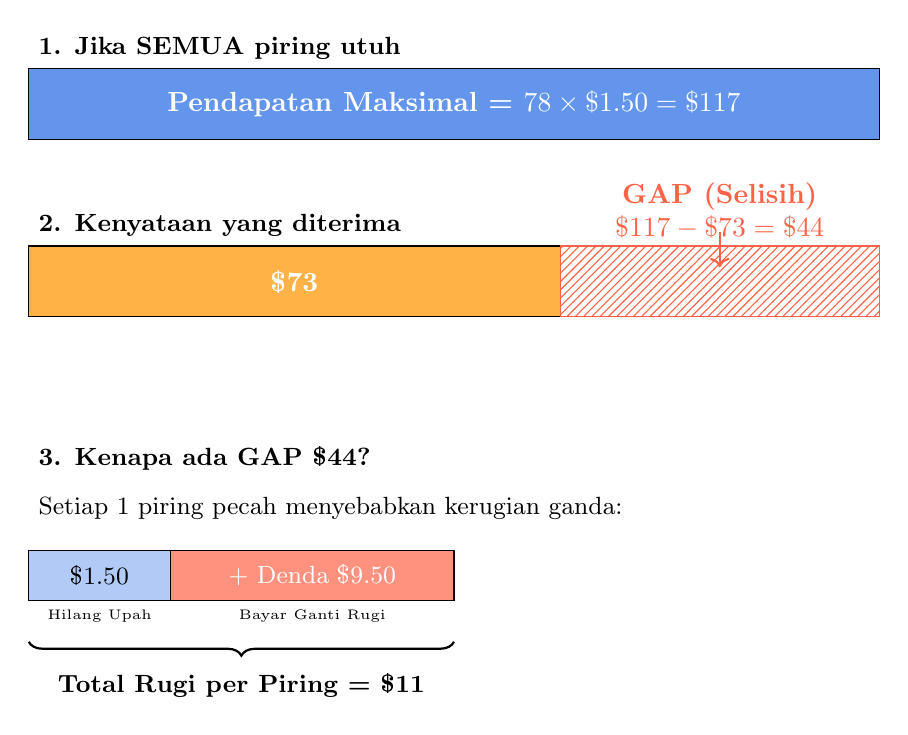
\begin{tikzpicture}[scale=0.9, every node/.style={font=\small}]
    % --- Bar 1: Harapan ---
    \node[anchor=south west] at (0, 3) {\textbf{1. Jika SEMUA piring utuh}};
    % Bar panjang (Biru)
    \draw[fill=colBlue, draw=black] (0, 2) rectangle (12, 3);
    \node[white, font=\bfseries] at (6, 2.5) {Pendapatan Maksimal = $78 \times \$1.50 = \$117$};

    % --- Bar 2: Kenyataan ---
    \node[anchor=south west] at (0, 0.5) {\textbf{2. Kenyataan yang diterima}};
    % Bar pendek (Oranye)
    \draw[fill=colOrange, draw=black] (0, -0.5) rectangle (7.5, 0.5);
    \node[white, font=\bfseries] at (3.75, 0) {\$73};

    % --- Bar Gap (Selisih) ---
    % Bar Arsiran Merah
    \draw[pattern=north east lines, pattern color=colRed, draw=colRed] (7.5, -0.5) rectangle (12, 0.5);
    \node[colRed, font=\bfseries, align=center] at (9.75, 1) {GAP (Selisih)\\$\$117 - \$73 = \$44$};
    \draw[->, thick, colRed] (9.75, 0.7) -- (9.75, 0.2); % Panah nunjuk ke gap

    % --- Penjelasan Unit Kerugian ---
    \node[anchor=west] at (0, -2.5) {\textbf{3. Kenapa ada GAP \$44?}};
    \node[anchor=west, align=left] at (0, -3.2) {Setiap 1 piring pecah menyebabkan kerugian ganda:};
    
    % Visualisasi 1 Unit Kerugian
    \draw[fill=colBlue!50, draw=black] (0, -4.5) rectangle (2, -3.8);
    \node at (1, -4.15) {\$1.50};
    \node[below, font=\tiny] at (1, -4.5) {Hilang Upah};
    
    \draw[fill=colRed!70, draw=black] (2, -4.5) rectangle (6, -3.8);
    \node[white] at (4, -4.15) {+ Denda \$9.50};
    \node[below, font=\tiny] at (4, -4.5) {Bayar Ganti Rugi};
    
    % Brace Total Rugi per Piring
    \draw[decorate,decoration={brace,amplitude=5pt,mirror,raise=15pt}, thick] (0, -4.5) -- (6, -4.5) 
    node[midway, below=0.8cm] {\textbf{Total Rugi per Piring = \$11}};

\end{tikzpicture}
\end{center}
\vspace{0.5cm}

\textbf{Hitungan:}
Total selisih uang (\$44) disebabkan oleh piring-piring yang pecah. Setiap satu piring pecah mengurangi total sebesar \$11.
\[ \text{Jumlah piring pecah} = \frac{\text{Total Selisih}}{\text{Rugi per Piring}} = \frac{44}{11} = \mathbf{4} \]

\end{document}
